Lexikální analyzátor je navržen a implementován jako deterministický ko\-neč\-ný automat, jehož graf přechodů je zobrazen na obrázku \ref{lex.lex}. Symbol \ae{} značí všechny ostatní symboly, pro které z daného stavu není jiný přechod.

\begin{figure}[h!]
\centering
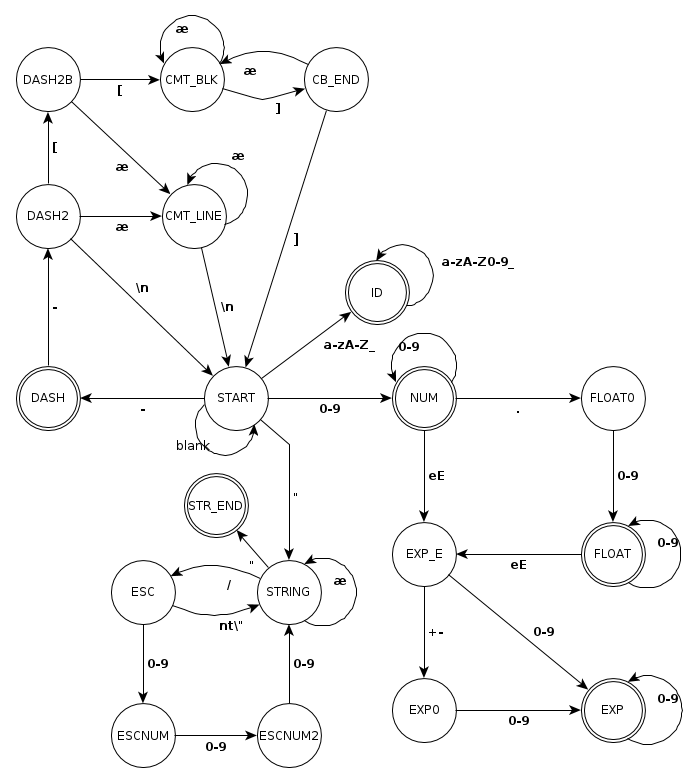
\includegraphics[width=11cm]{lexical.png}
\caption{Schéma konečného automatu lexikálního analyzátoru}
\label{lex.lex}
\end{figure}

V koncovém stavu pro indentifikátory skončí i klíčová a rezervovaná slova. Kdyby je měl automat zpracovávat zvlášť, přibylo by mnoho stavů a automat by se stal nepřehledným. Proto jsou zpracovány společně s identifikátory a na konci je volána funkce, která určí, zda se skutečně jedná o identifikátor, nebo některé z klíčových nebo rezervovaných slov.

Graf na obázku \ref{lex.lex} není úplný, nepopisuje celý automat, ale jen jeho část, která analyzuje řetězce, identifikátory, čísla a komentáře. Analýza ostatních lexémů, jedná se o operátory, je realizována jen jedním, případně dvěma, přechody z počátečního stavu {\tt start}. Graf by se ale při takovém množství přechodů z počátečního stavu stal nepřehledným. Proto je pro úplnost zpracování operátorů zobrazeno na obrázku \ref{lex.ope} bokem od složitější a zajímavější části automatu z obrázku \ref{lex.lex}.

\begin{figure}
\centering
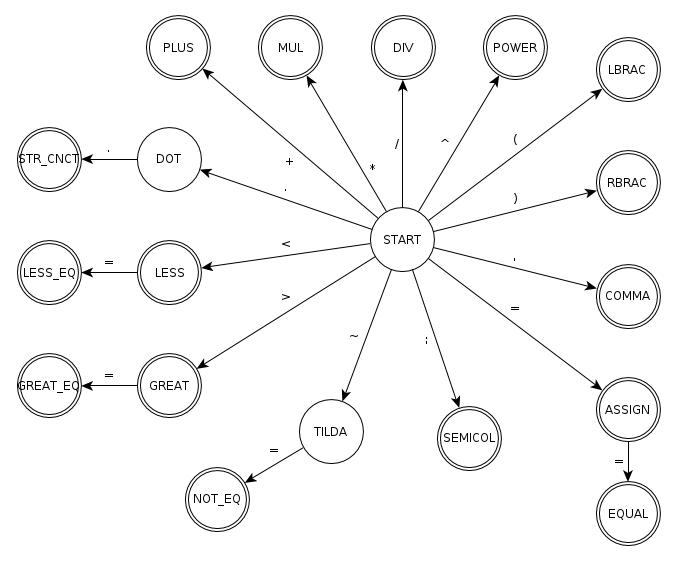
\includegraphics[width=10cm]{operator.png}
\caption{Schéma konečného automatu lexikálního analyzátoru}
\label{lex.ope}
\end{figure}
